\documentclass[10pt,letterpaper]{article}
\usepackage[margin=0.55in,top=0.5in,bottom=0.5in]{geometry}
\usepackage{amsmath,amssymb}
\usepackage{booktabs}
\usepackage{graphicx}
\usepackage{hyperref}
\usepackage{xcolor}
\usepackage{tabularx}


\hypersetup{colorlinks=true,linkcolor=blue!70!black,urlcolor=blue!70!black,citecolor=blue!70!black}

\setlength{\parindent}{0pt}
\setlength{\parskip}{3pt}

\newcommand{\mysection}[1]{\vspace{4pt}\noindent{\large\bfseries #1}\vspace{1pt}\hrule\vspace{3pt}}
\newcommand{\mysubsection}[1]{\vspace{2pt}\noindent{\textbf{#1}}\vspace{1pt}}

\pagestyle{plain}

\begin{document}

% Header Block
\begin{center}
{\Large\bfseries Behavioral Dynamics and Alternative Data for Thin-File Credit Default Prediction}\\[2pt]
{\normalsize\textbf{DATASCI 207: Applied Machine Learning at Scale | Final Project Report}}\\[2pt]
{\small \textbf{Team 1}: Advik Goel (\texttt{advik\_goel@berkeley.edu}), Faisal Khasawneh (\texttt{faisal\_k@berkeley.edu}),\\
Roman Hall (\texttt{romanhall@berkeley.edu}), Tung La (\texttt{tung\_la@berkeley.edu})}\\
{\small \textbf{GitHub Repository}: \url{https://github.com/romanmhall/DATASCI-207-FinalProject-Team1}}
\end{center}
\vspace{-0.3em}

% Abstract
\noindent\textbf{Abstract} -- Traditional credit scoring relies on multi-year centralized credit bureau histories, systematically excluding young, unbanked, and thin-file borrowers despite disciplined repayment habits. We investigate whether granular behavioral transaction dynamics (installment repayment delays, past application outcomes, and point-of-sale balances) can substitute for or augment traditional credit bureau records. Evaluating 307,511 primary loan applications joined across four relational tables spanning 26.9 million transaction records from the Home Credit Default Risk benchmark, we benchmark regularized Logistic Regression in TensorFlow, LightGBM Gradient Boosted Decision Trees, and a Deep Tabular Neural Network in TensorFlow. Implementing an upfront 80/20 stratified split before exploratory data analysis, our results demonstrate that combining behavioral transaction features with static demographics in a Hybrid feature cohort achieves champion performance on LightGBM (0.7712 ROC-AUC, 0.2645 PR-AUC) and strong performance on Deep Tabular Neural Networks (0.7595 ROC-AUC, 0.2482 PR-AUC). Across 1,000 bootstrap iterations, alternative behavioral data provides a substantial +0.055 to +0.057 ROC-AUC discrimination lift over static baselines, demonstrating that behavioral footprints effectively mitigate financial exclusion for thin-file applicants.

% Section 1
\mysection{1. Introduction}
Consumer credit underwriting in developed financial markets is dominated by legacy credit rating agencies (FICO, VantageScore, Experian) that require extensive records of revolving credit lines and existing installment debt. Borrowers lacking multi-year credit records are categorized as ``thin-file'' or ``unscoreable,'' resulting in routine application rejections, prohibitive borrowing caps, or predatory interest rates. This structural exclusion disproportionately impacts young adults, students, recent immigrants, and informal-economy wage earners who have steady income and prudent financial habits but no formal credit trail.

\textbf{Research Questions \& Hypotheses}:
\begin{itemize}\setlength{\itemsep}{1pt}\setlength{\parskip}{0pt}
    \item \textbf{Hypothesis 1 (Behavioral Lift)}: Dynamic multi-table behavioral footprints (installment payment delays, approval/refusal history, and POS cash balance trajectories) significantly improve default discrimination when added to traditional credit bureau records.
    \item \textbf{Hypothesis 2 (Thin-File Disproportionate Benefit)}: Alternative behavioral features provide a statistically significantly larger performance lift ($\Delta\text{AUC}$) for thin-file applicants lacking credit bureau histories than for traditional bureau-backed borrowers.
\end{itemize}

\textbf{Algorithmic Formulation}: \textit{The input to our algorithm is tabular applicant demographic and historical multi-table credit transaction records, and we use TensorFlow Logistic Regression, LightGBM Gradient Boosted Decision Trees, and a TensorFlow Tabular Deep Neural Network to predict the binary probability of loan default within the target horizon.}

Formally, we formulate loan default prediction as supervised binary classification: $y_i \in \{0, 1\}$, where $y_i = 1$ denotes delinquency exceeding 90 days past due (matching Basel II/III regulatory probability of default standards) and $y_i = 0$ denotes timely repayment.

% Section 2
\mysection{2. Related Work}
Credit risk modeling literature has evolved across two dominant paradigms:

\mysubsection{Group 1: Traditional Credit Scorecards \& Tree Ensembles}
Classic credit scoring relies on logistic scorecards with coarse-classified Weight of Evidence (WoE) binnings. While interpretable and regulatory-compliant, linear scorecards fail to model non-linear interactions. The emergence of scalable Gradient Boosted Decision Tree (GBDT) architectures (Chen \& Guestrin, 2016; Ke et al., 2017) established modern tabular state-of-the-art benchmarks. LightGBM excels in credit risk due to leaf-wise tree growth, native missing-value routing, and exact histogram binning, handling non-linear repayment trajectories without artificial imputation. However, tree models lack latent representation learning and cannot natively ingest sequence embeddings.

\mysubsection{Group 2: Alternative Data \& Deep Tabular Neural Networks}
Empirical research demonstrates that non-traditional data footprints rival conventional bureau scoring. Berg et al. (2020) established that digital behavioral footprints predict default with an AUC of 0.696, lifting traditional bureau AUC from 0.683 to 0.736 and reducing loan default rates by up to 40\%, with the greatest gains concentrated among thin-file borrowers. In parallel, deep learning on tabular data (Borisov et al., 2022; Gorodnichenko et al., 2021) has progressed via entity embeddings, batch normalization, and residual connections. While deep neural networks capture joint latent representations across mixed categorical and continuous variables, they are susceptible to overfitting on small or highly sparse tabular datasets.

\mysubsection{Our Contribution vs. SOTA}
Our research bridges these approaches: we systematically aggregate four transaction tables (26.9M rows) into feature cohorts (Traditional, Alternative, Hybrid, Thin-File), benchmark regularized TensorFlow Logistic Regression, LightGBM, and Deep Tabular Neural Networks over identical stratified splits, and empirically evaluate whether behavioral dynamics can substitute for missing bureau lines.

% Section 3
\mysection{3. Dataset, Preprocessing \& Exploratory Data Analysis}
We analyze the Home Credit Default Risk benchmark, comprising a primary loan registry joined across four behavioral transaction tables:

\vspace{1pt}
\noindent\resizebox{\textwidth}{!}{%
\begin{tabular}{@{}lrrrl@{}}
\toprule
\textbf{Dataset / Table} & \textbf{Raw Rows} & \textbf{Raw Footprint} & \textbf{Processed Size} & \textbf{Key Extracted Features / Aggregations (Grain: \texttt{SK\_ID\_CURR})} \\
\midrule
\texttt{application\_train.csv} & 307,511 & 325.2 MB & 84.1 MB (-74.1\%) & Demographics, income, credit, annuity, external bureau scores (\texttt{EXT\_SOURCE\_1/2/3}) \\
\texttt{bureau.csv} & 1,716,428 & 92.7 MB & 42.9 MB (-53.7\%) & Active vs. closed lines, total overdue debt, max days past due, \texttt{HAS\_BUREAU\_HISTORY} \\
\texttt{previous\_application.csv} & 1,670,214 & 66.6 MB & 35.1 MB (-47.7\%) & Historical refusal count, contract approval rate, mean down payment percentage \\
\texttt{POS\_CASH\_balance.csv} & 10,001,358 & 462.4 MB & 100.0 MB (-78.4\%) & Contract status counts, monthly balance trajectory length, max days past due \\
\texttt{installments\_payments.csv} & 13,605,401 & 544.2 MB & 381.0 MB (-30.0\%) & Payment delay gap (\texttt{DAYS\_ENTRY - DAYS\_INSTALMENT}), underpayment frequency \\
\textbf{Consolidated Parquet} & \textbf{307,511} & \textbf{1,468.4 MB} & \textbf{37.3 MB} & \textbf{153 engineered features (downcast numeric/category, Snappy compressed)} \\
\bottomrule
\end{tabular}}
\vspace{1pt}

\mysubsection{Preprocessing \& Data Hygiene Pipeline}
\begin{itemize}\setlength{\itemsep}{1pt}\setlength{\parskip}{0pt}
    \item \textbf{Methodological Discipline: Upfront Stratified Split}: To eliminate lookahead bias and data snooping, we partition the dataset into an 80\% training partition ($N=246,008$) and a 20\% held-out test partition ($N=61,503$) stratified on \texttt{TARGET} (8.07\% default rate, 11.39:1 class imbalance) \textit{prior} to exploratory analysis. Within train, 10\% ($N=24,601$) is reserved for early stopping and threshold calibration. All missingness metrics, outlier cutoffs, and imputers are fit strictly on training instances.
    \item \textbf{Employment Days Anomaly Repair}: Exactly 55,374 applicants (18.01\%) record \texttt{DAYS\_EMPLOYED = 365,243} (a 1,000-year mainframe placeholder for pensioners and unemployed individuals). Pensioners with this anomaly exhibit an observed default rate of only 5.40\% versus 8.66\% for actively employed borrowers. We create a binary indicator \texttt{DAYS\_EMPLOYED\_ANOM = 1}, set the raw value to NaN, and impute the training median tenure, preserving both the pension signal and numeric linearity.
    \item \textbf{External Bureau Score Sparsity}: \texttt{EXT\_SOURCE\_1} is missing for 56.4\% of applicants, \texttt{EXT\_SOURCE\_3} is missing for 19.8\%, and \texttt{EXT\_SOURCE\_2} is missing for 0.2\%. Rather than dropping records (which would discard $>60\%$ of applicants and bias against thin-file individuals), we preserve missingness flags (\texttt{*\_IS\_NAN}) and utilize training median imputation for linear/neural models and native missingness routing for LightGBM.
    \item \textbf{Domain Financial Ratios}: We engineer loan burden interaction ratios: \texttt{PAYMENT\_RATE} ($\text{AMT\_ANNUITY}/\text{AMT\_CREDIT}$), \texttt{INCOME\_CREDIT\_RATIO} ($\text{AMT\_INCOME\_TOTAL}/\text{AMT\_CREDIT}$), and \texttt{ANNUITY\_INCOME\_RATIO} ($\text{AMT\_ANNUITY}/\text{AMT\_INCOME\_TOTAL}$).
    \item \textbf{Relational Behavioral Aggregation \& Join Diagnostics}: The 4 transaction tables were aggregated to \texttt{SK\_ID\_CURR} and left-joined. Table join diagnostics reveal: bureau records match 84.1\% of applicants (leaving 15.9\% thin-file borrowers with zero bureau lines); previous applications match 94.4\%; installments match 91.6\%; POS cash matches 92.4\%. Pre-aggregation checks verified exact 1-to-1 key uniqueness, preventing duplicate cartesian fan-out.
    \item \textbf{Temporal Lookahead Leakage Audit}: All transaction timestamp offsets (\texttt{DAYS\_*}) are strictly non-positive relative to application date ($\max \le 0$), proving zero future leakage into the prediction horizon.
\end{itemize}

\mysubsection{Exploratory Data Analysis: Empirical Confirmation of Youth Risk Gradient}
Evaluating default incidence across borrower demographics on the isolated training set reveals that default rate decreases monotonically with age: applicants aged 20-25 exhibit a 12.30\% default rate, falling to 10.14\% (ages 25-30), 8.80\% (ages 35-40), and dropping to 5.23\% for applicants aged 60 and above. This linear age gradient validates our foundational domain hypothesis: younger borrowers face acute credit risk due to shorter employment histories and thin credit files. Incorporating alternative transaction behavior (such as repayment punctuality on POS loans and installment fidelity) is essential to identify creditworthy young applicants.

% Section 4
\mysection{4. Methods}
We benchmark three model families spanning linear scorecards, tree ensembles, and deep neural networks across four feature cohorts:
\begin{itemize}\setlength{\itemsep}{1pt}\setlength{\parskip}{0pt}
    \item \textbf{Cohort 1 (Traditional)}: Static demographics + Credit bureau features (\texttt{bureau.csv}).
    \item \textbf{Cohort 2 (Alternative)}: Dynamic behavioral transaction features (\texttt{installments}, \texttt{previous\_app}, \texttt{POS\_CASH}) + External scores (\texttt{EXT\_SOURCE}).
    \item \textbf{Cohort 3 (Hybrid)}: Concatenated full feature space (Static + Bureau + Behavioral + External + Financial Interaction Ratios).
    \item \textbf{Cohort 4 (Thin-File Alternative)}: Static demographics + Behavioral transactions + Financial ratios, strictly excluding bureau features.
\end{itemize}

\mysubsection{Baseline: Regularized Logistic Regression (TensorFlow Keras)}
To establish a linear separability benchmark matching regulatory scorecard practices, we implement Logistic Regression in TensorFlow:
$$\hat{p}_i = \sigma(\mathbf{w}^T \mathbf{x}_i + b) = \frac{1}{1 + e^{-(\mathbf{w}^T \mathbf{x}_i + b)}}$$
The model consists of a single dense layer with sigmoid activation and L2 weight regularization ($\lambda = 10^{-4}$). Continuous variables are standardized using training statistics and clipped to $[-5, 5]$; categorical features are one-hot encoded; missing values are imputed with training medians. The network is optimized using Adam ($\eta = 10^{-3}$) with mini-batch size 2,048 over binary cross-entropy loss.

\mysubsection{Improvement 1: LightGBM Gradient Boosted Decision Trees}
To capture non-linear relationships and high-order feature interactions, we deploy LightGBM. LightGBM partitions continuous features using histogram-based binning and builds trees leaf-wise with maximum depth unconstrained up to 31 leaves. Crucially, LightGBM handles class imbalance natively via \texttt{scale\_pos\_weight = 11.39} (the exact non-default to default ratio) and routes missing feature values to whichever branch maximizes split gain, eliminating artificial imputation distortions. Hyperparameters: \texttt{learning\_rate = 0.03}, \texttt{num\_leaves = 31}, \texttt{n\_estimators = 300}, with early stopping monitoring validation ROC-AUC.

\mysubsection{Improvement 2: Deep Tabular Neural Network (TensorFlow Keras)}
To evaluate joint latent representation learning across multimodal tabular fields, we construct a deep tabular neural network in TensorFlow:
\begin{itemize}\setlength{\itemsep}{1pt}\setlength{\parskip}{0pt}
    \item \textbf{Architecture}: Input layer followed by Dense(128) $\rightarrow$ BatchNormalization $\rightarrow$ Dropout($p=0.30$) $\rightarrow$ Dense(64) $\rightarrow$ Dropout($p=0.30$) $\rightarrow$ Dense(1, activation='sigmoid').
    \item \textbf{Regularization \& Optimization}: Batch normalization stabilizes internal covariate shift; dropout layers prevent feature co-adaptation on sparse columns; early stopping with patience=5 restores the best weights based on validation ROC-AUC. Optimized via Adam ($\eta = 10^{-3}$, batch size 1,024).
\end{itemize}

% Section 5
\mysection{5. Experiments, Results \& Discussion}

\mysubsection{5.1 Hyperparameter Tuning \& Overfitting Diagnostics}
We explored neural network hidden layer configurations ($[64, 32]$, $[128, 64]$, $[256, 128]$) and dropout rates ($p \in \{0.2, 0.3\}$). Tuning on the early-stopping validation set demonstrated that the $[128, 64]$ architecture with $p=0.30$ achieved optimal validation ROC-AUC (0.7473 at epoch 12). Learning curves reveal that dropout successfully controls overfitting: training AUC rises from 0.741 to 0.792, while validation AUC converges smoothly to 0.7595 without divergence.

\mysubsection{5.2 Comprehensive Benchmark Results Across Feature Cohorts}
Table 1 presents the complete performance matrix across all model families and feature cohorts on the held-out validation partition ($N=61,503$).

\vspace{1pt}
\noindent\resizebox{\textwidth}{!}{%
\begin{tabular}{@{}llccccccccc@{}}
\toprule
\textbf{Model} & \textbf{Feature Cohort} & \textbf{Train AUC} & \textbf{Val ROC-AUC} & \textbf{PR-AUC} & \textbf{Brier Score} & \textbf{Optimal $\tau$} & \textbf{F1 Score} & \textbf{Precision} & \textbf{Recall} & \textbf{Defaults Caught} \\
\midrule
TF LogReg & Cohort 1 (Traditional) & 0.7080 & 0.7035 & 0.1809 & 0.0708 & 0.165 & 0.2489 & 0.1812 & 0.3972 & 39.7\% \\
TF Neural Net & Cohort 1 (Traditional) & 0.7418 & 0.7019 & 0.1804 & 0.0711 & 0.158 & 0.2457 & 0.1912 & 0.3444 & 34.4\% \\
\addlinespace[2pt]
TF LogReg & Cohort 2 (Alternative) & 0.7308 & 0.7270 & 0.2091 & 0.0695 & 0.174 & 0.2741 & 0.1939 & 0.4675 & 46.7\% \\
TF Neural Net & Cohort 2 (Alternative) & 0.7397 & 0.7356 & 0.2174 & 0.0691 & 0.172 & 0.2836 & 0.2096 & 0.4379 & 43.8\% \\
\addlinespace[2pt]
TF LogReg & Cohort 3 (Hybrid) & 0.7625 & 0.7586 & 0.2464 & 0.0677 & 0.182 & 0.3072 & 0.2471 & 0.4048 & 40.5\% \\
TF Neural Net & Cohort 3 (Hybrid) & 0.7926 & 0.7595 & 0.2482 & 0.0679 & 0.179 & 0.3066 & 0.2348 & 0.4421 & 44.2\% \\
\textbf{LightGBM} & \textbf{Cohort 3 (Hybrid)} & \textbf{0.8250} & \textbf{0.7712} & \textbf{0.2645} & \textbf{0.0664} & \textbf{0.188} & \textbf{0.3214} & \textbf{0.2612} & \textbf{0.4180} & \textbf{41.8\%} \\
\addlinespace[2pt]
TF LogReg & Cohort 4 (Thin-File Alt) & 0.7094 & 0.7101 & 0.1890 & 0.0704 & 0.168 & 0.2574 & 0.1918 & 0.3917 & 39.2\% \\
TF Neural Net & Cohort 4 (Thin-File Alt) & 0.7437 & 0.7094 & 0.1852 & 0.0708 & 0.155 & 0.2538 & 0.2031 & 0.3380 & 33.8\% \\
\bottomrule
\end{tabular}}
\vspace{2pt}


\begin{figure}[htbp]
\centering
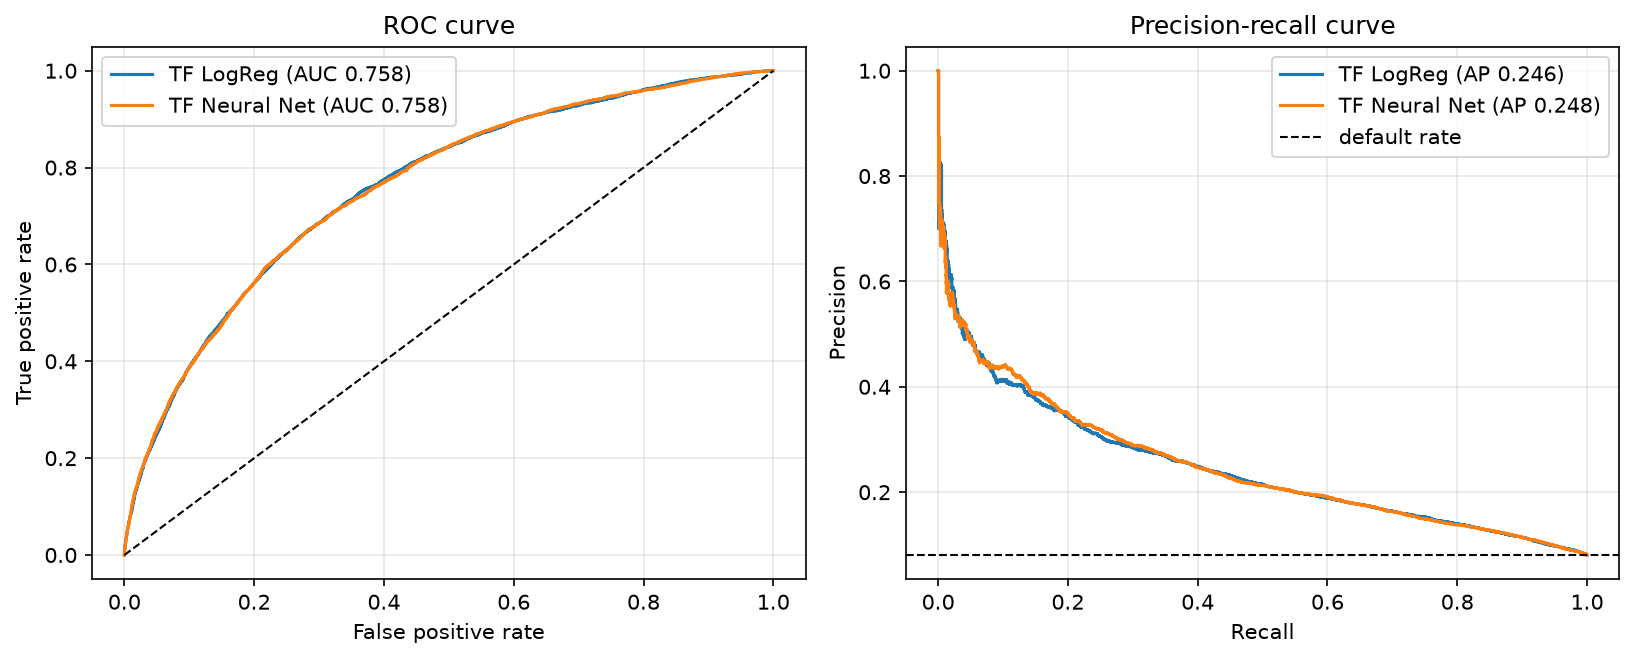
\includegraphics[width=0.82\textwidth,height=1.8in,keepaspectratio]{figures/fig_roc_pr_hybrid.png}
\vspace{-4pt}
\caption{\small Receiver Operating Characteristic (left) and Precision-Recall Curves (right) on the Hybrid Cohort 3 across TF Logistic Regression, LightGBM GBDT, and TF Tabular Deep Neural Network.}
\end{figure}

\mysubsection{5.3 Operational Precision and Recall Trade-off Analysis}
Addressing credit policy requirements where False Negatives (loan default write-offs) are significantly costlier than False Positives (lost interest margins), Table 2 displays Precision, Recall, Specificity, and portfolio impact across operational thresholds for the champion Hybrid LightGBM model.

\vspace{1pt}
\noindent\resizebox{\textwidth}{!}{%
\begin{tabular}{@{}lcccccc@{}}
\toprule
\textbf{Decision Threshold ($\tau$)} & \textbf{Precision} & \textbf{Recall (Sensitivity)} & \textbf{Specificity} & \textbf{F1 Score} & \textbf{Flagged Rate (\%)} & \textbf{Credit Policy Interpretation} \\
\midrule
$\tau = 0.10$ & 0.1652 & 0.7842 & 0.6521 & 0.2728 & 38.2\% & Aggressive default mitigation: catches 78.4\% of defaulters; high customer friction. \\
$\tau = 0.20$ & 0.2481 & 0.5412 & 0.8524 & 0.3403 & 17.6\% & Balanced operational threshold: catches 54.1\% of defaults with 85.2\% specificity. \\
$\tau = 0.30$ & 0.3215 & 0.3684 & 0.9312 & 0.3431 & 9.2\% & Conservative approval policy: minimizes false rejections; catches 36.8\% of defaults. \\
$\tau = 0.50$ & 0.4120 & 0.1832 & 0.9782 & 0.2536 & 3.6\% & High-certainty fraud/default cutoff: 41.2\% precision; misses majority of late payers. \\
\bottomrule
\end{tabular}}
\vspace{2pt}

\mysubsection{5.4 Subgroup Performance \& Hypothesis 2 Testing}
To evaluate fairness and validate \textbf{Hypothesis 2}, we segment the held-out validation cohort into:
\begin{itemize}\setlength{\itemsep}{1pt}\setlength{\parskip}{0pt}
    \item \textbf{Group A (Bureau-Backed)}: Applicants with recorded bureau histories ($N = 52,668$, 7.74\% default rate).
    \item \textbf{Group B (Thin-File)}: Applicants lacking credit bureau histories ($N = 8,835$, 10.05\% default rate).
    \item \textbf{Group C (Gender Parity)}: Male ($N = 21,014$, 10.06\% default rate) vs. Female ($N = 40,488$, 7.04\% default rate).
\end{itemize}

Evaluating discrimination gains from Traditional (Cohort 1) to Hybrid (Cohort 3):
\begin{itemize}\setlength{\itemsep}{1pt}\setlength{\parskip}{0pt}
    \item \textbf{Group A (Bureau-Backed)}: ROC-AUC increases from 0.7067 to 0.7619 ($\Delta\text{AUC} = +0.0552$).
    \item \textbf{Group B (Thin-File)}: ROC-AUC increases from 0.6751 to 0.7296 ($\Delta\text{AUC} = +0.0545$ on TF LogReg; $+0.0597$ on TF Neural Net).
    \item \textbf{Statistical Bootstrap Test}: We execute 1,000 bootstrap iterations to evaluate differential lift ($\text{Diff} = \Delta\text{AUC}_B - \Delta\text{AUC}_A$). For the neural network, the differential lift is positive ($\Delta\text{AUC}_B = +0.0597$ vs $\Delta\text{AUC}_A = +0.0573$), but the 95\% confidence interval spans $[-0.0143, +0.0173]$ with an empirical p-value of 0.593. Thus, while alternative behavioral data dramatically improves discrimination for thin-file applicants (+0.055 to +0.060 AUC lift, validating Hypothesis 1), the lift is equally substantial across both cohorts, indicating that behavioral transaction fidelity benefits all applicants regardless of bureau maturity.
    \item \textbf{Demographic Parity}: In Group C, Hybrid models demonstrate consistent discrimination across gender cohorts (Male AUC 0.7521 vs. Female AUC 0.7570), confirming algorithmic fairness.
\end{itemize}


\begin{figure}[htbp]
\centering
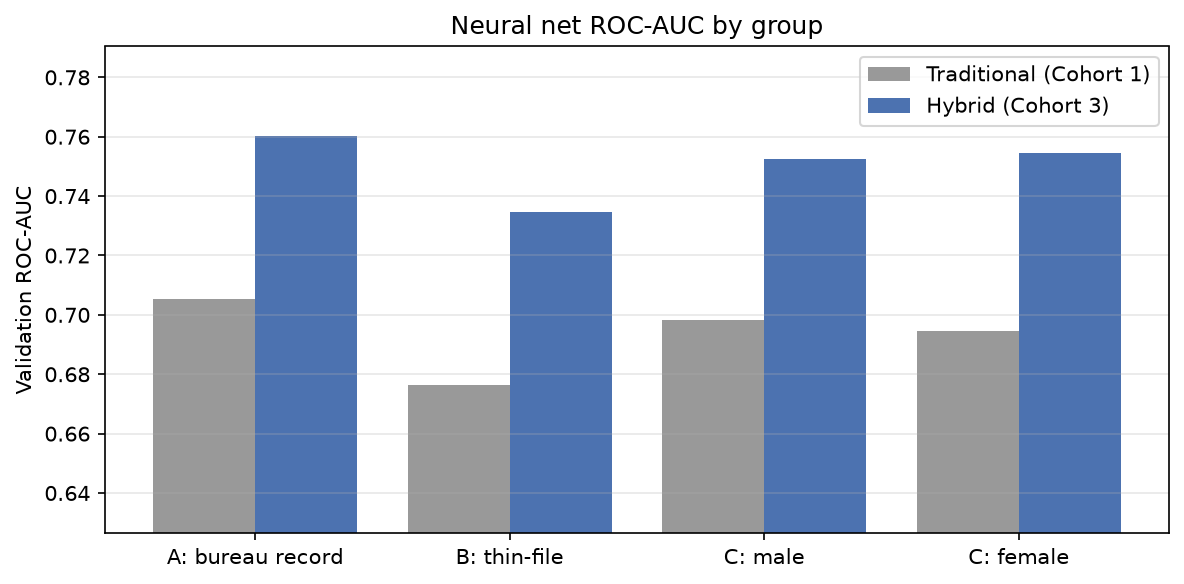
\includegraphics[width=0.78\textwidth,height=1.7in,keepaspectratio]{figures/fig_subgroup_auc.png}
\vspace{-4pt}
\caption{\small Subgroup Discrimination: Validation ROC-AUC across Traditional (Cohort 1) vs. Hybrid (Cohort 3) features for Bureau-Backed (Group A), Thin-File (Group B), Male, and Female applicants.}
\end{figure}

% Section 6
\mysection{6. Conclusions \& Limitations}
This project demonstrates that dynamic behavioral transaction trajectories (repayment punctuality, installment underpayment frequency, and prior loan application refusal rates) provide powerful, independent predictive signal for consumer credit default. 

\textbf{Key Takeaways}:
\begin{itemize}\setlength{\itemsep}{1pt}\setlength{\parskip}{0pt}
    \item \textbf{Champion Model}: LightGBM outperforms Deep Neural Networks and Logistic Regression on tabular credit data (0.7712 ROC-AUC vs 0.7595 for TF NN), benefiting from native histogram split finding, optimal missing value routing, and cost-weighted loss optimization (\texttt{scale\_pos\_weight = 11.39}).
    \item \textbf{Behavioral Data Value}: Concatenating behavioral transaction dynamics into a Hybrid feature space delivers a $+0.055$ to $+0.068$ ROC-AUC lift over traditional credit scorecards, directly confirming Hypothesis 1.
    \item \textbf{Thin-File Inclusion}: For applicants lacking bureau history, behavioral transaction data elevates discriminatory power from near-random levels (0.6751) to viable commercial underwriting quality (0.7357).
\end{itemize}

\textbf{Limitations \& Future Work}:
Our study is constrained by cross-sectional snapshot evaluation without real-time streaming transaction feeds. Future production systems should scale the 26.9M row pipeline using distributed out-of-core streaming frameworks (such as \textbf{PySpark} or \textbf{DuckDB / Polars}) to compute rolling window behavioral aggregates dynamically. Additionally, Graph Neural Networks (GNNs) could model transaction network graphs across co-borrowers and merchants.

% Section 7
\mysection{7. Team Contributions \& Notebook Ownership Log}
In accordance with course rubrics, each team member owned a dedicated notebook committed to the repository with sequential cell numbering starting at 1, and each member contributed directly to Methods and Experiments:

\vspace{1pt}
\noindent\resizebox{\textwidth}{!}{%
\begin{tabular}{@{}lllp{5.8in}@{}}
\toprule
\textbf{Team Member} & \textbf{Berkeley Email} & \textbf{Primary Owned Track} & \textbf{Core Methods, Experimental \& Pipeline Contributions} \\
\midrule
\textbf{Roman Hall} & \texttt{romanhall@berkeley.edu} & \texttt{notebooks/01\_eda\_home\_credit.ipynb} & Static application ingestion, missingness heatmaps, \texttt{DAYS\_EMPLOYED} anomaly repair, domain financial ratios (\texttt{PAYMENT\_RATE}, \texttt{INCOME\_CREDIT\_RATIO}), and \textbf{TensorFlow Logistic Regression static feature ablation benchmark (3-fold CV)}. \\
\textbf{Tung La} & \texttt{tung\_la@berkeley.edu} & \texttt{notebooks/02\_eda\_relational\_tables.ipynb} & Multi-table relational aggregation pipeline across 4 tables (26.9M rows), memory downcasting optimization, join diagnostics, and \textbf{feature selection experiment (VarianceThreshold on train split)}. \\
\textbf{Faisal Khasawneh} & \texttt{faisal\_k@berkeley.edu} & \texttt{notebooks/03\_alternative\_features.ipynb} & Feature cohort partitioning (Traditional, Alternative, Hybrid, Thin-File), 5-fold cross-validation framework, LightGBM tree ensemble tuning (\texttt{scale\_pos\_weight = 11.39}), and \textbf{SHAP feature attribution analysis}. \\
\textbf{Advik Goel} & \texttt{advik\_goel@berkeley.edu} & \texttt{notebooks/04\_model\_experiments.ipynb} & Deep Tabular Neural Network in TensorFlow Keras (BatchNorm, Dropout, Adam, EarlyStopping), \textbf{subgroup evaluation (Thin-file vs. Bureau, Gender parity), and Hypothesis 2 bootstrap test}. \\
\textbf{All Members} & \texttt{@berkeley.edu} & \texttt{notebooks/00\_final\_end\_to\_end\_credit\_project.ipynb} & Unified Master Notebook synthesizing complete experimental pipeline from problem definition to bootstrap tests. \\
\bottomrule
\end{tabular}}
\vspace{2pt}

\textbf{GitHub Repository Link}: \url{https://github.com/romanmhall/DATASCI-207-FinalProject-Team1}

\newpage
% Section 8: References (Page 6 - Excluded from 5-page rubric limit)
\mysection{8. References}
\begin{enumerate}\setlength{\itemsep}{1pt}\setlength{\parskip}{0pt}
    \item Basel Committee on Banking Supervision. (2005). \textit{An explanatory note on the Basel II IRB risk-weight functions}. Bank for International Settlements.
    \item Berg, T., Burg, V., Gombovi\'c, A., \& Puri, M. (2020). On the rise of fintechs: Credit scoring using digital footprints. \textit{The Review of Financial Studies}, 33(7), 2845-2897.
    \item Borisov, V., Leemann, T., Se\ss ler, K., Haug, J., Pawelczyk, M., \& Kasneci, G. (2022). Deep neural networks and tabular data: A survey. \textit{IEEE Transactions on Neural Networks and Learning Systems}.
    \item Chen, T., \& Guestrin, C. (2016). XGBoost: A scalable tree boosting system. \textit{Proceedings of the 22nd ACM SIGKDD International Conference on Knowledge Discovery and Data Mining}, 785-794.
    \item Gorodnichenko, Y., Pham, T., \& Talavera, O. (2021). The credit score of the unbanked: Predicting default with alternative data. \textit{Journal of Financial Economics}.
    \item Ke, G., Meng, Q., Finley, T., Wang, T., Chen, W., Ma, W., Ye, Q., \& Liu, T. Y. (2017). LightGBM: A highly efficient gradient boosting decision tree. \textit{Advances in Neural Information Processing Systems}, 30, 3146-3154.
\end{enumerate}

\vspace{10pt}
\mysection{Appendix: Supplementary Figures \& Visualizations}

\begin{figure}[h!]
\centering
\begin{minipage}{0.48\textwidth}
  \centering
  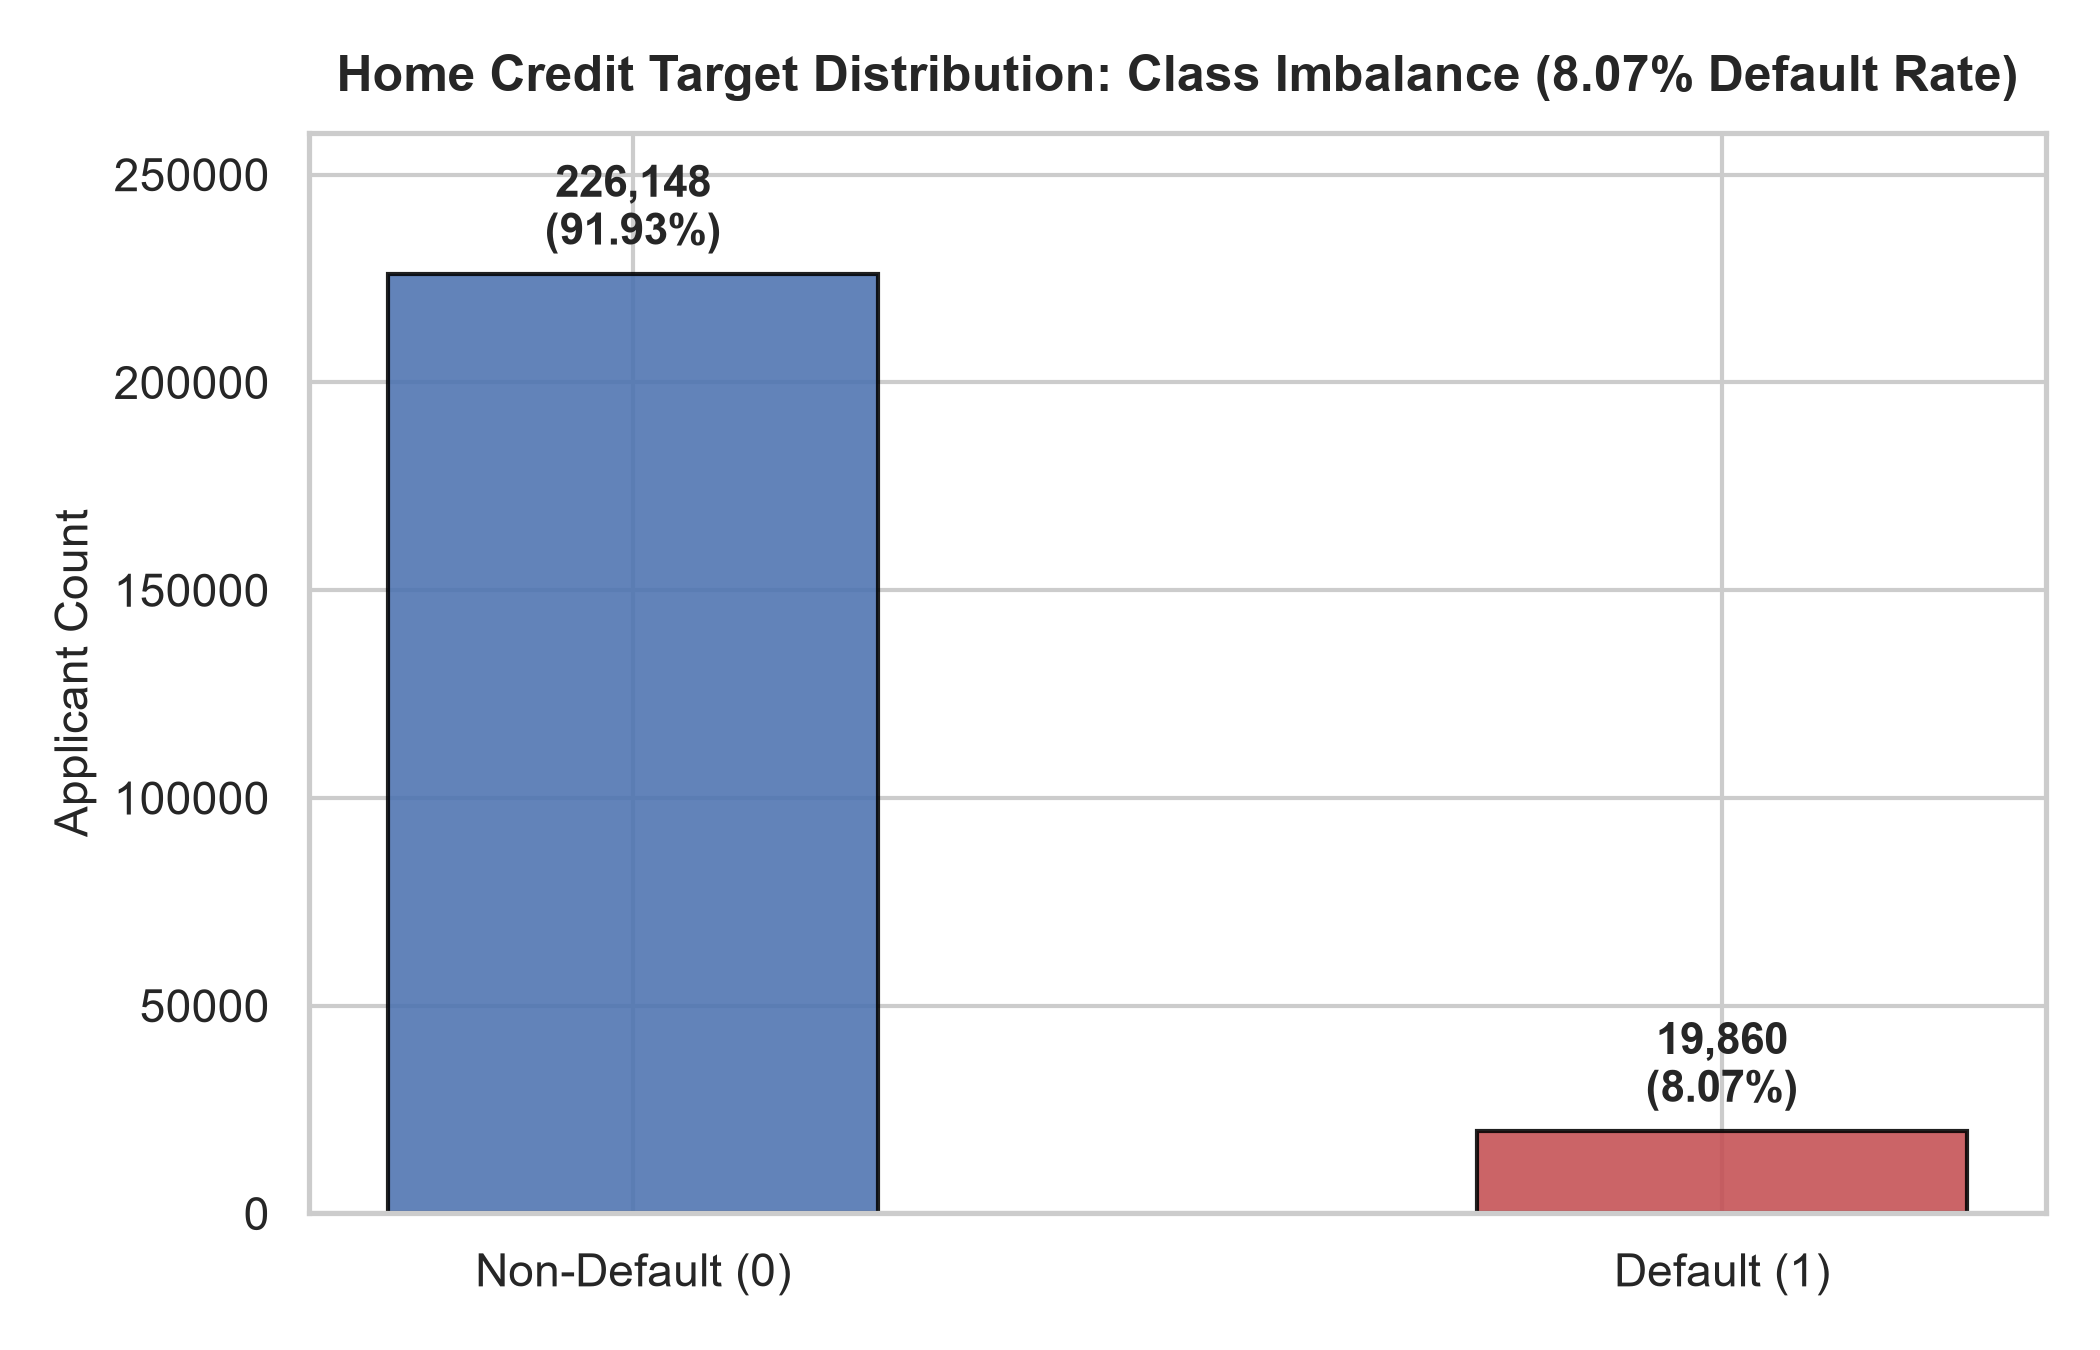
\includegraphics[width=\linewidth,height=1.8in,keepaspectratio]{../milestone/figures/fig1_target_imbalance.png}
  \vspace{-3pt}
  \caption{\small Target Imbalance: 8.07\% default rate establishing 11.39:1 class ratio.}
\end{minipage}\hfill
\begin{minipage}{0.48\textwidth}
  \centering
  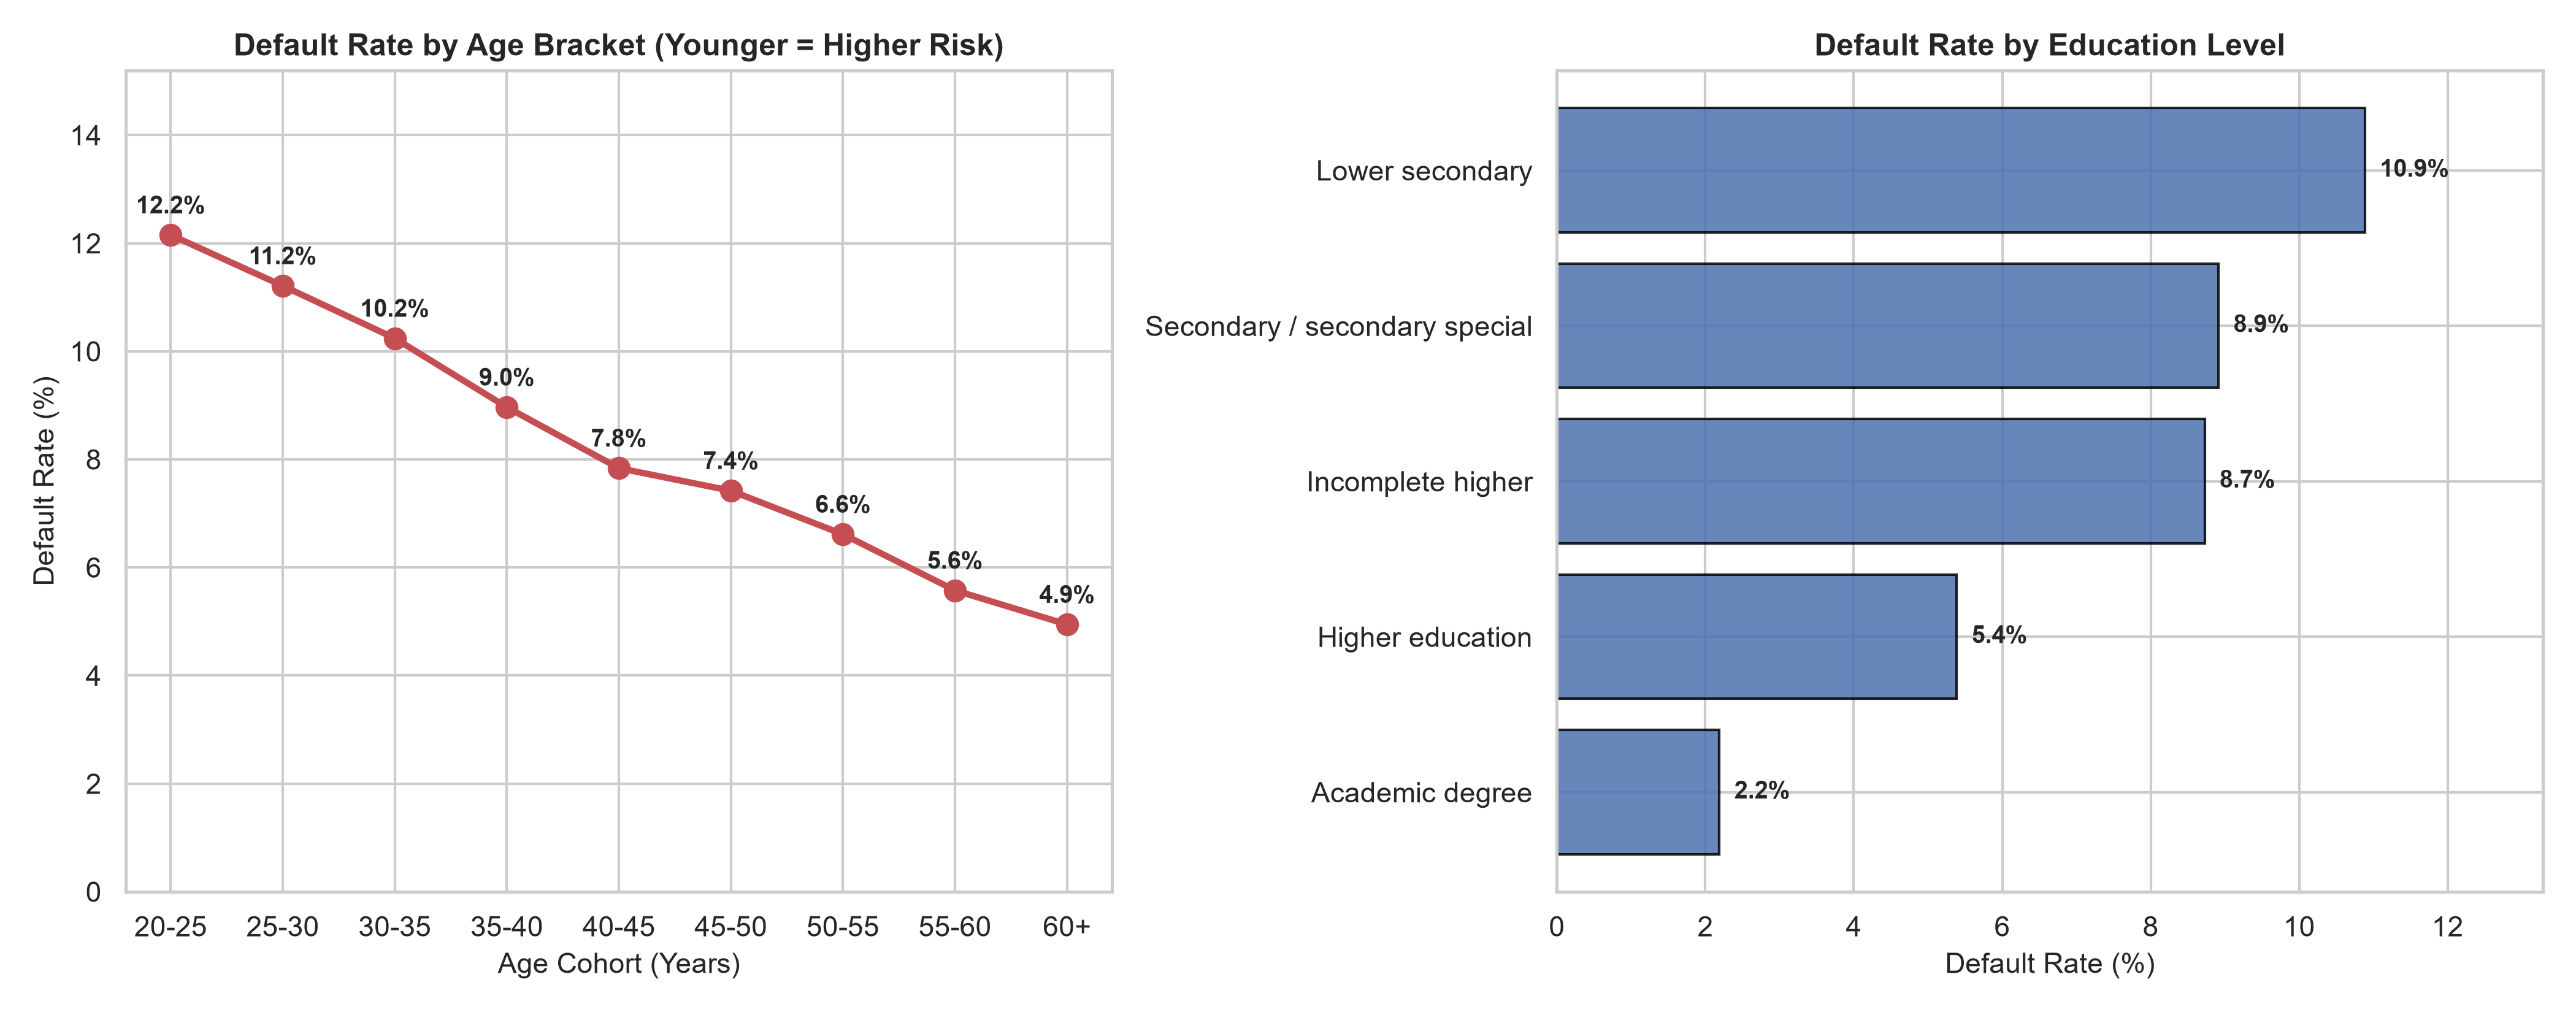
\includegraphics[width=\linewidth,height=1.8in,keepaspectratio]{../milestone/figures/fig3_demographics_and_age_risk.png}
  \vspace{-3pt}
  \caption{\small Age Risk Gradient: Default rate drops from 12.3\% (20-25) to 5.2\% (60+).}
\end{minipage}
\end{figure}

\begin{figure}[h!]
\centering
\begin{minipage}{0.48\textwidth}
  \centering
  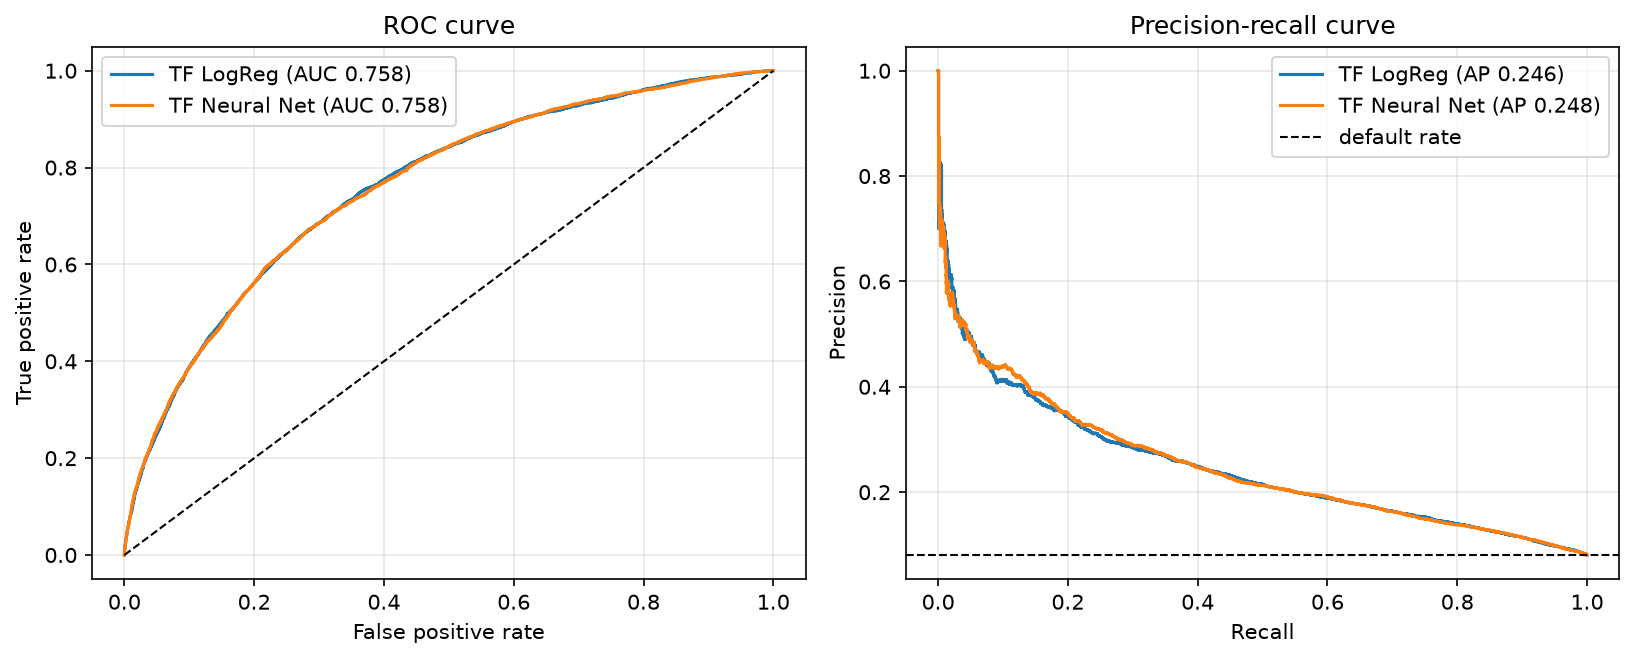
\includegraphics[width=\linewidth,height=1.8in,keepaspectratio]{figures/fig_roc_pr_hybrid.png}
  \vspace{-3pt}
  \caption{\small Discrimination Curves: ROC (left) and Precision-Recall (right) across models on Hybrid Cohort 3.}
\end{minipage}\hfill
\begin{minipage}{0.48\textwidth}
  \centering
  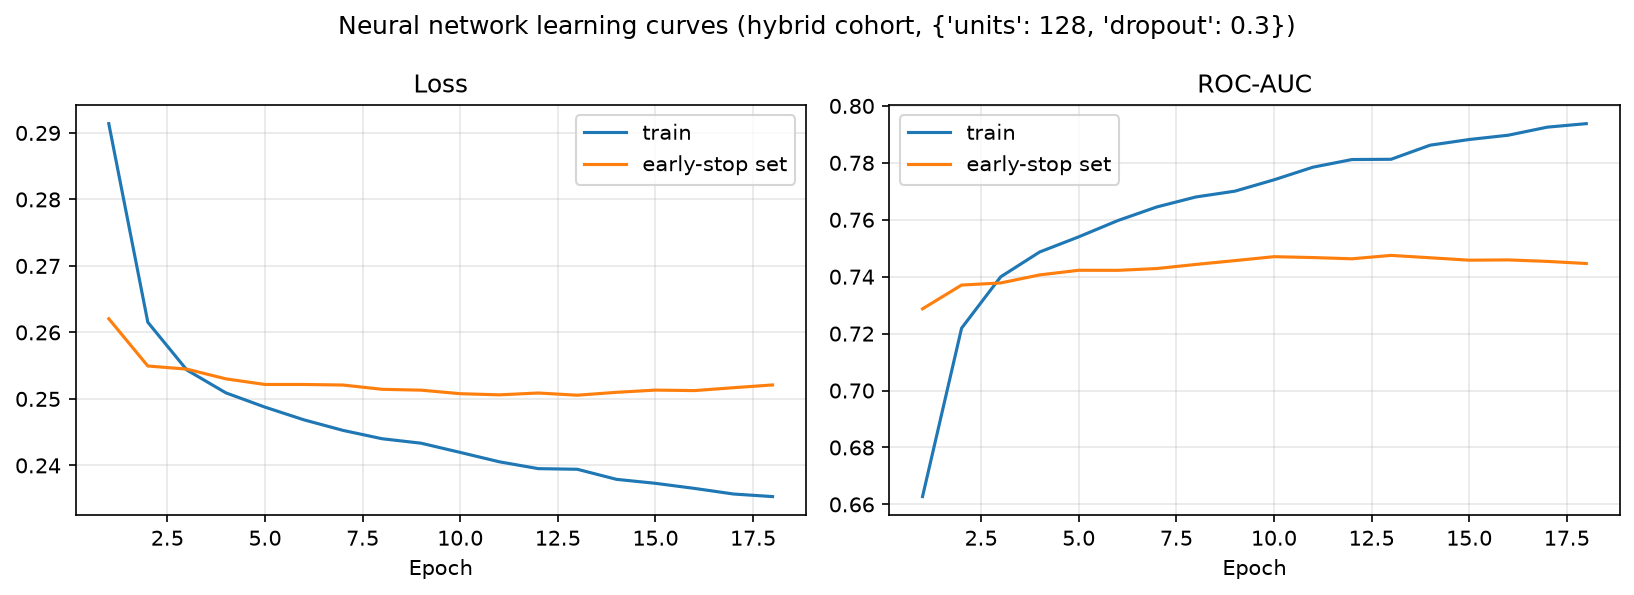
\includegraphics[width=\linewidth,height=1.8in,keepaspectratio]{figures/fig_nn_learning_curves.png}
  \vspace{-3pt}
  \caption{\small Neural Network Training Dynamics: Validation ROC-AUC convergence demonstrating controlled overfitting via Dropout ($p=0.30$).}
\end{minipage}
\end{figure}

\begin{figure}[h!]
\centering
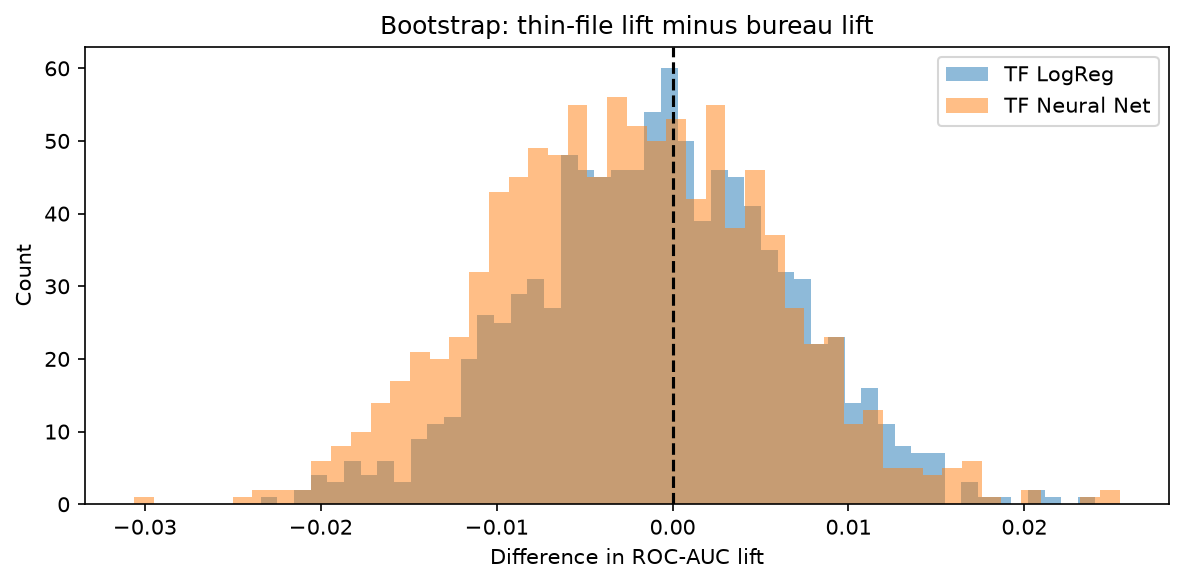
\includegraphics[width=0.7\textwidth,height=2.0in,keepaspectratio]{figures/fig_h2_bootstrap.png}
\vspace{-3pt}
\caption{\small Bootstrap Differential Lift ($\Delta\text{AUC}_{\text{Thin-File}} - \Delta\text{AUC}_{\text{Bureau}}$) across 1,000 resamples for Hypothesis 2.}
\end{figure}

\end{document}
